\documentclass[tikz,border=10pt]{standalone}

\usepackage{tikz}
\usetikzlibrary{shapes}


\begin{document}

\begin{tikzpicture}

 \node at (0, 3)   (input) {input};    
 \node[draw] at (0, 2.5)   (a) {$0\,1\,0\,1\,1\,0\,1\,0\,1$};    
    
\node[inner sep=0pt] (russell) at (0,0)
    {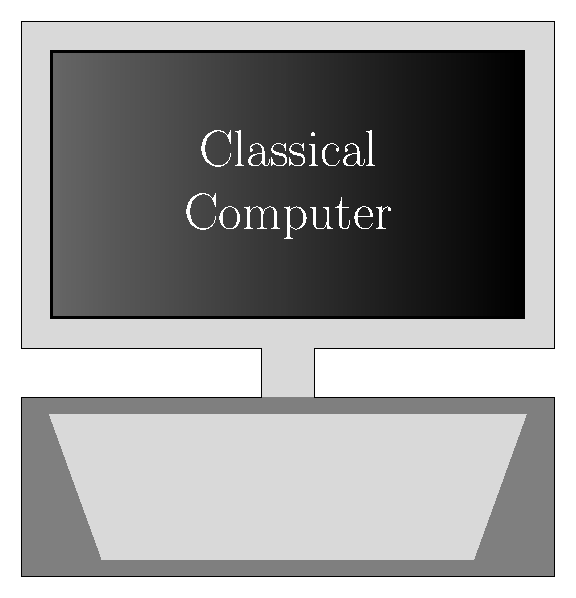
\includegraphics[width=.25\textwidth]{ClassicalComputer.pdf}};

\node[draw] at (0, -2.5)   (b) {$1\,1\,0\,1\,1\,0\,0\,1\,0$};   
 \node at (0, -3)   (input) {output};    
 
\draw[->,thick] (0,2.2) -- (0,1.5);

\draw[->,thick] (0,-1.5) -- (0,-2.2);

%\node[inner sep=0pt] (bottom) at (0,-6)
%    {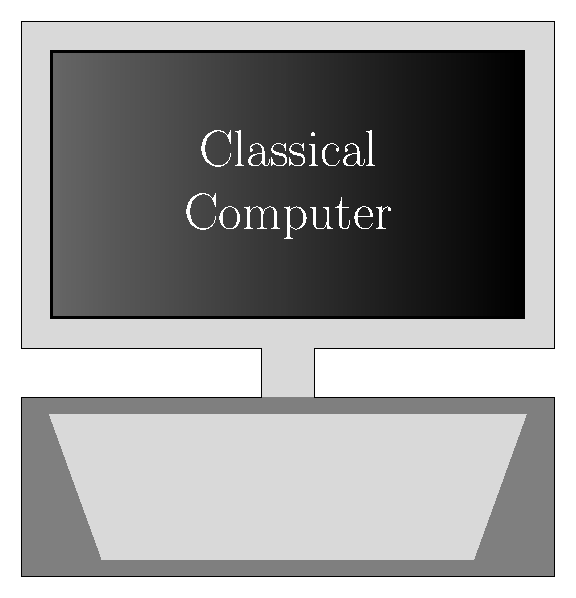
\includegraphics[width=.25\textwidth]{ClassicalComputer.pdf}};
 
%\draw[<->,thick] (russell.south east) -- (bottom.center);
%    
%\draw[<->,thick] (russell.center) -- (bottom.center)
%    node[midway,fill=white] {Principia Mathematica};
 
 %Node

  
\end{tikzpicture}


\end{document}